\section{Experiment}
\subsection{Test Bench}
We use MiBench \cite{guthaus2001mibench} as our test bench for injecting faults and evaluating our system. MiBench is a representative embedded benchmark. We choose MiBench because of its compact program size and versatile program characteristics. We choose qsort as our test program.

\subsection{Metrics}
we use Precision-Recall (PR) curve and $F_1$ score as our evaluation criteria. More precisely, we have
\begin{equation}
F_{1} = 2\cdot\frac{precision \cdot recall}{precision + recall},
\end{equation}
where $precision = \frac{tp}{tp+fp}$, $recall = \frac{tp}{tp+fn}$, $tp$ is the number true positive samples, $fp$ is number of false positive samples, and $fn$ is the number of false negative samples. For multi-class classification, we use confusion matrix to describe the performance of our classifier.

\subsection{Experiment Setups}
Here are our four experiment setups: 1) same input data with all features, 2) same input data with handpicked subsets of features, 3) different input data with all meaningful features, and 4) different input data with handpicked subsets of features.

\section{Result}
\subsection{Same Input All Features}
(same input all features SIAF)

\begin{figure}[t]
\begin{center}
   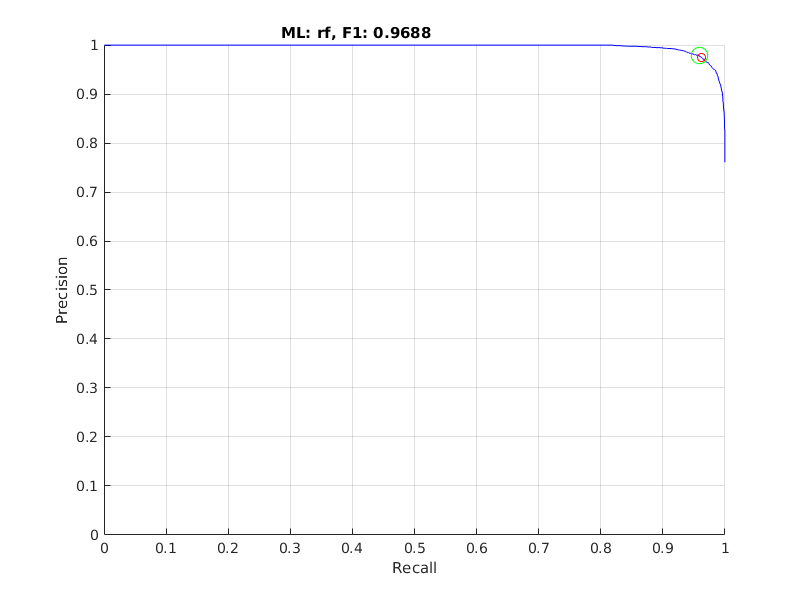
\includegraphics[width=0.95\linewidth]{./figures/siaf.png}
\end{center}
   \caption{}
\label{fig:siaf}
\end{figure}

\begin{figure}[t]
\begin{center}
   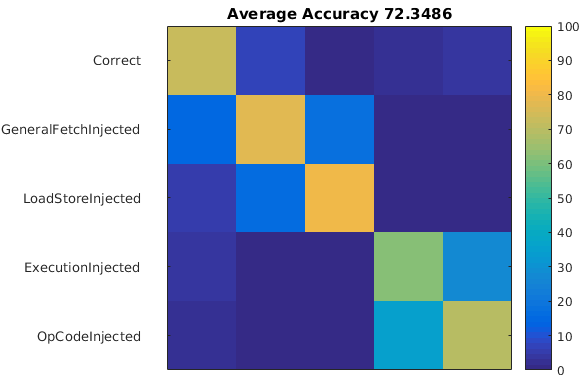
\includegraphics[width=0.95\linewidth]{./figures/siaf_multi.png}
\end{center}
   \caption{}
\label{fig:siaf-multi}
\end{figure}

The random forest algorithm output the importance score of each feature based on its discriminative power. The importance feature ranking is depicted in Figure~\ref{fig:feat-same}.
\begin{figure}[t]
\begin{center}
   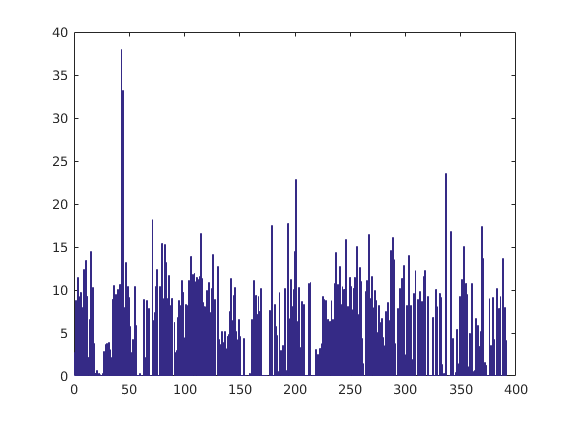
\includegraphics[width=0.95\linewidth]{./figures/feat_same.png}
\end{center}
   \caption{}
\label{fig:feat-same}
\end{figure}

\subsection{Same Input Different Features}
(same input handpicked features SIHF)

\begin{figure}[t]
\begin{center}
   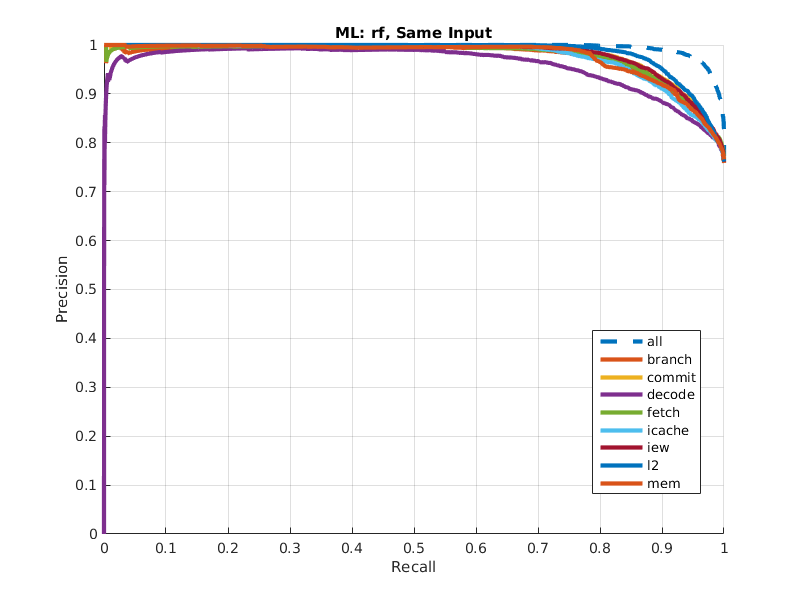
\includegraphics[width=0.95\linewidth]{./figures/sidf.png}
\end{center}
   \caption{}
\label{fig:sidf}
\end{figure}

\subsection{Different Input All Features}
(different input all features DIAF)

\begin{figure}[t]
\begin{center}
   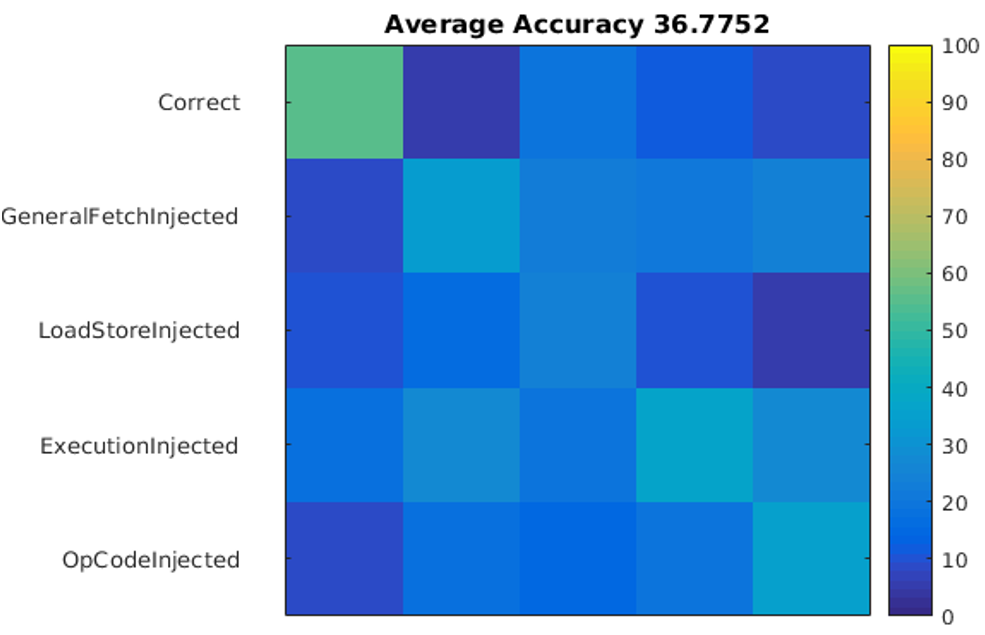
\includegraphics[width=0.95\linewidth]{./figures/diaf_multi.png}
\end{center}
   \caption{}
\label{fig:diaf-multi}
\end{figure}

\begin{figure}[t]
\begin{center}
   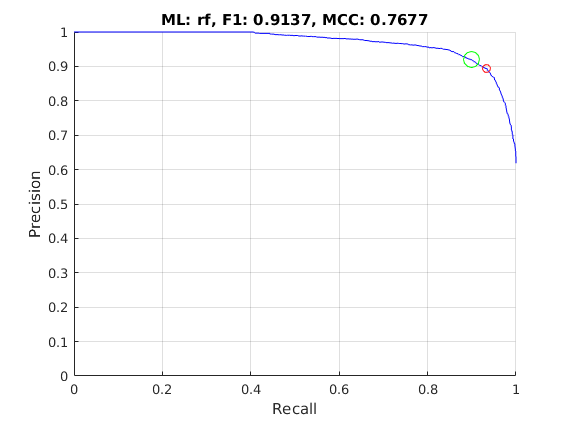
\includegraphics[width=0.95\linewidth]{./figures/disf.png}
\end{center}
   \caption{}
\label{fig:disf}
\end{figure}

\begin{figure}[t]
\begin{center}
   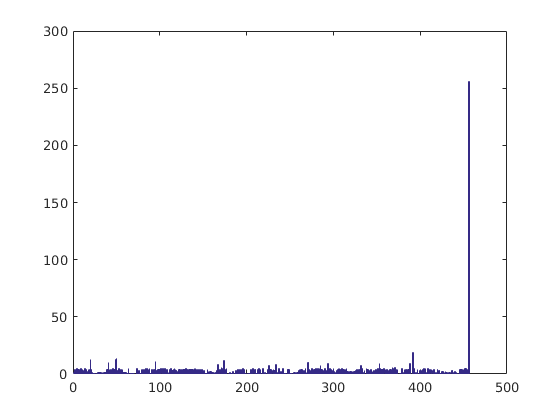
\includegraphics[width=0.95\linewidth]{./figures/feat_diff.png}
\end{center}
   \caption{}
\label{fig:feat-diff}
\end{figure}

\subsection{Different Input Different Features}
Different Input Handpicked Features DIHF

\begin{figure}[t]
\begin{center}
   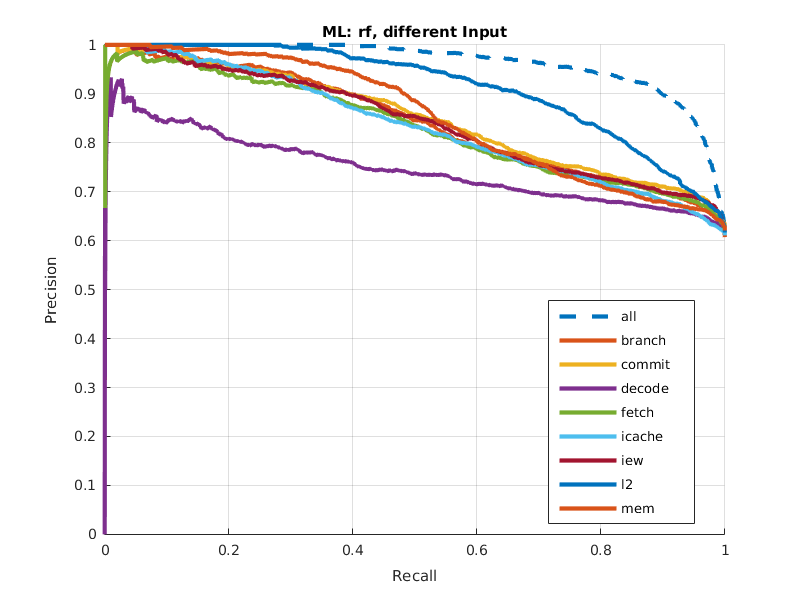
\includegraphics[width=0.95\linewidth]{./figures/didf.png}
\end{center}
   \caption{}
\label{fig:didf}
\end{figure}

\subsection{Cross Application Predication}
